\documentclass[sigconf]{acmart}

\usepackage{booktabs}
\graphicspath{{../../figures/statistics/}{../../figures/machine_learning/}}

\copyrightyear{2026}
\acmYear{2026}
\setcopyright{rightsretained}
\acmConference[ML Course Project]{Machine Learning Course Project}{2026}{UNAM, Morelia, Mexico}
\acmDOI{}
\acmISBN{}

\setcitestyle{square}
\settopmatter{authorsperrow=2}

\begin{document}
\sloppy

\title[Predicting Video Game Sales and Genre]{Predicting Video Game Sales and Genre Using Machine Learning}

\author{Adrian Lara}
\affiliation{%
  \department{Information Technologies for Sciences}
  \institution{National Autonomous University of Mexico (UNAM)}
  \city{Morelia}
  \country{Mexico}}
\email{adrianlarasc@gmail.com}

\renewcommand{\shortauthors}{Adrian Lara}

\begin{abstract}
This project applies three supervised machine learning algorithms: Decision Tree, Logistic Regression, and Naive Bayes to the
Video Game Sales dataset (vgsales) sourced from Kaggle. The dataset was previously engineered with additional features including \texttt{Publisher\_Tier},
\texttt{Genre\_Group}, \texttt{Platform\_Gen}, \texttt{Sales\_Tier}, and \texttt{Decade}, which we will use for our analysis. The Decision Tree and Logistic Regression models
were trained to predict \texttt{Sales\_Tier}, while the Naive Bayes model was trained to predict \texttt{Genre\_Group}. While Decision Tree and Logistic Regression
achieved results that may seem low, they provided valuable insights on the nature of the data and the impact of class imbalance on an extremely right-skewed dataset.
Naive Bayes performed poorly, which can be attributed to the violation of its independence assumption. Class imbalance was
identified as a central challenge, but I still wanted to explore its effects with this project, as this dataset also gave a very interesting statistics project.
For reference, here's a view of the distribution of the sales in this dataset, along with the distribution of the transformed Sales variable using log1p:
\end{abstract}

\maketitle

\begin{figure}[ht]
  \centering
  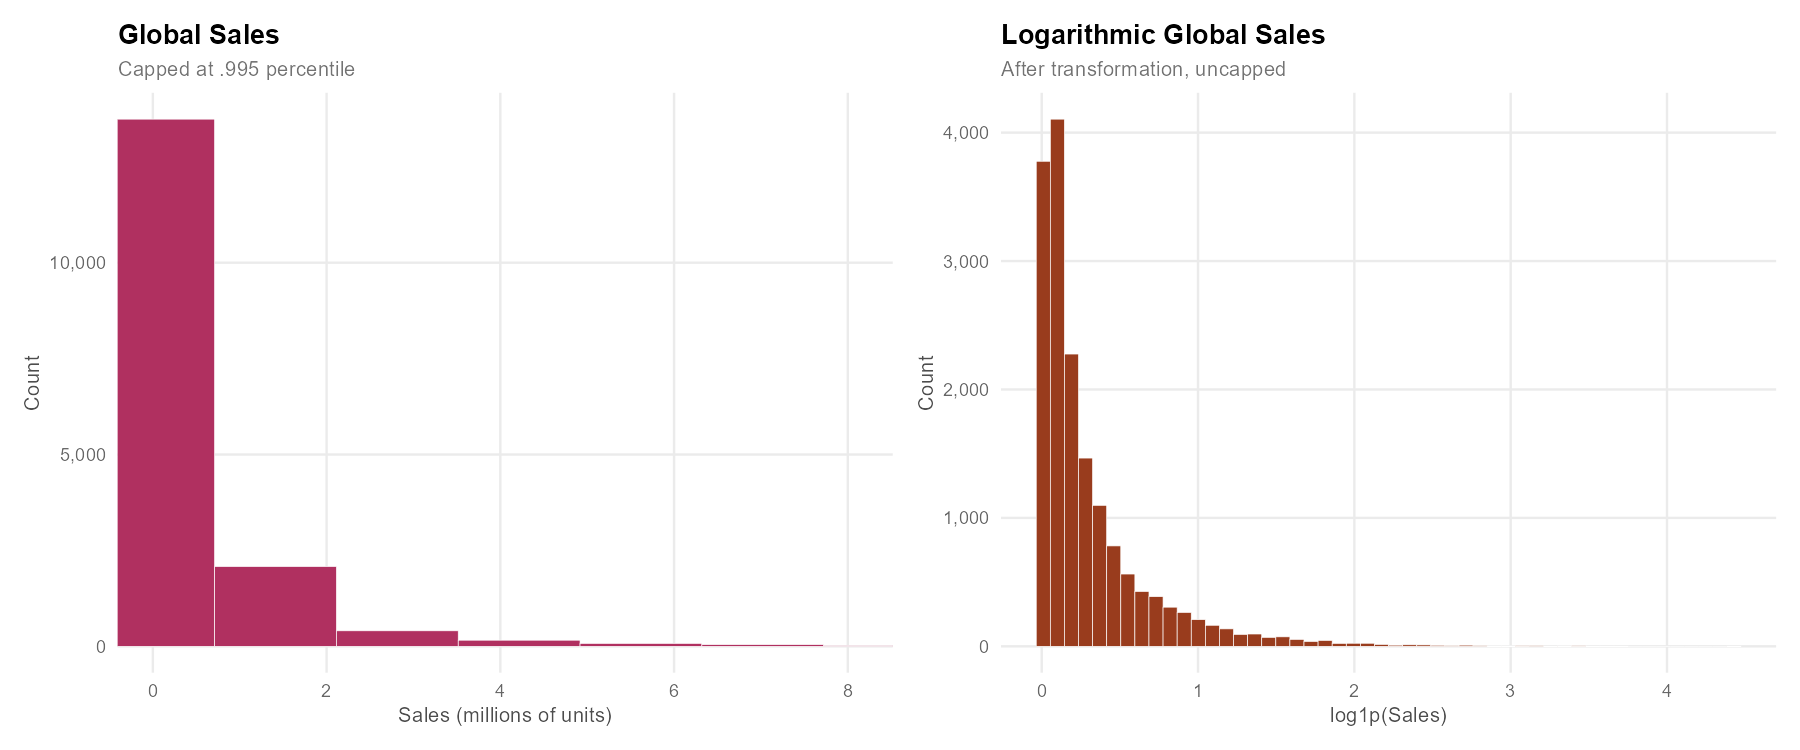
\includegraphics[width=\linewidth]{p1_distributions}
  \caption{Distribution of \texttt{Global\_Sales} (left) and log-transformed \texttt{Global\_Sales} (right).}
\end{figure}

\section{Introduction}

The video game industry is a multi-billion dollar market with a highly competitive landscape. Predicting the sales performance of videogames is a
highly complex task influenced by a multitude of factors. In this project, we explore the application of three supervised machine learning models
to determine how well we can predict a game's sales tier and genre based on a set of engineered features like decade, platform generation, and publisher tier.

The dataset used is the Video Game Sales dataset (vgsales) from Kaggle, which contains over 16,000 entries with regional and global sales figures
for games released between the 1980s and the 2010s.

Three classification algorithms were selected for this study: Decision Tree, Logistic Regression, and Naive Bayes. Each model was chosen for
its interpretability. A key objective of this project is not only to compare model accuracy, but to understand \textit{why} each model behaves the way it does, including its failures.

\section{Dataset and Feature Engineering}

\subsection{Original Dataset}

The raw vgsales dataset contains the following columns: \texttt{Rank}, \texttt{Name}, \texttt{Platform}, \texttt{Year}, \texttt{Genre},
\texttt{Publisher}, \texttt{NA\_Sales}, \texttt{EU\_Sales}, \texttt{JP\_Sales}, \texttt{Other\_Sales}, and \texttt{Global\_Sales}.
Sales values are expressed in millions of units sold.

Missing values were handled in the preprocessing step (written in R): the 271 missing \texttt{Year} values were imputed with the median
release year of the game's platform, and the 58 missing \texttt{Publisher} values were labelled \texttt{"Unknown"}.

\subsection{Engineered Features}

Five new variables were derived from the original columns to improve model performance and interpretability.

\textbf{Publisher\_Tier} groups the original 578 publishers by number of games into three categories: \textit{Major} (top 10),
\textit{Mid} (ranks 11--50), and \textit{Small} (the rest). This reduces sparsity.

\textbf{Genre\_Group} consolidates the original 12 genres into the top 7 most frequent genres plus an \textit{Other} category.

\textbf{Platform\_Gen} maps each platform to its hardware generation, ranging from Gen3-4 through Gen8, plus a \textit{PC/Other} category for PC and niche platforms.

\textbf{Sales\_Tier} bins \texttt{Global\_Sales} into four ordinal categories: \textit{Niche}, \textit{Moderate},
\textit{Hit}, and \textit{Blockbuster}. Niche was engineered according to the games below the median, while the others were engineered according
to personal perception of the sales tiers.

\textbf{Decade} derives the release decade from the \texttt{Year} column, yielding four categories: 1980s, 1990s, 2000s, and 2010s.

\subsection{Class Imbalance}

A significant class imbalance was identified in \texttt{Sales\_Tier}.
The vast majority of games fall into the \textit{Niche} and \textit{Moderate} categories, while \textit{Hit}
accounts for very little results along \textit{Blockbuster}. This imbalance poses a challenge for model training.

\section{Methodology}

\subsection{Experimental Setup}

All three models were trained and evaluated using Python's \texttt{scikit-learn} library. The dataset was split into 80\%
training and 20\% testing using stratified sampling to preserve class proportions in both sets (\texttt{random\_state=42}). Hyperparameter
tuning was performed using \texttt{GridSearchCV} with 5-fold cross-validation on the training set.

\subsection{Decision Tree}

The Decision Tree classifier was trained to predict \texttt{Sales\_Tier} using \texttt{Publisher\_Tier}, \texttt{Genre\_Group},
\texttt{Platform\_Gen}, and \texttt{Decade} as features. All features were ordinal-encoded inside a \texttt{Pipeline}. \texttt{GridSearchCV} was used to search over \texttt{max\_depth}
(1--20), \texttt{min\_samples\_split} (5, 10), and \texttt{criterion} (\textit{gini}, \textit{entropy}). Two trees were tuned: an unweighted
tree selected by accuracy, and a tree with \texttt{class\_weight="balanced"} selected by \emph{balanced accuracy} (the mean recall over the
four classes). Tuning the weighted tree by plain accuracy would defeat its purpose, since accuracy rewards predicting the majority class.

\subsection{Logistic Regression}

Logistic Regression was also trained to predict \texttt{Sales\_Tier} on the same feature set, enabling direct comparison with the Decision
Tree. Features were one-hot encoded via \texttt{OneHotEncoder} and scaled with \texttt{StandardScaler} inside a \texttt{Pipeline} to
prevent data leakage. The regularization parameter \texttt{C} was tuned via \texttt{GridSearchCV} across six values (0.001 to 100) on a
log scale, using balanced accuracy as the selection metric. Multinomial logistic regression was used with the \texttt{lbfgs} solver and
\texttt{class\_weight="balanced"}.

\subsection{Naive Bayes}

The Naive Bayes model was trained to predict \texttt{Genre\_Group}. \texttt{CategoricalNB} was selected over \texttt{GaussianNB} because
all features \texttt{Publisher\_Tier}, \texttt{Platform\_Gen}, \texttt{Sales\_Tier}, and \texttt{Decade} are discrete categories
with no continuous distribution. Features were encoded with \texttt{OrdinalEncoder}. The smoothing parameter \texttt{alpha} was
tuned via \texttt{GridSearchCV} across seven values (0.01 to 10), using accuracy as the selection metric.

\section{Results}

\subsection{Decision Tree}

Without class weighting, the best tree (\texttt{max\_depth}=9, \textit{gini}) achieved 56\% accuracy but predicted \textit{Blockbuster}
with zero recall, effectively ignoring the rarest class, and recalled only 7\% of \textit{Hit} games. With \texttt{class\_weight="balanced"}
(best \texttt{max\_depth}=11), overall accuracy dropped to 40\%, but balanced accuracy rose from 0.33 to 0.41: recall for
\textit{Blockbuster} improved from 0.00 to 0.54 and recall for \textit{Hit} from 0.07 to 0.33.

The decision tree visualization below shows the first three levels of the balanced tree; its first split is on \texttt{Publisher\_Tier}.
In the unweighted tree, \texttt{Publisher\_Tier} (importance 0.41) and \texttt{Platform\_Gen} (0.28) were the most influential predictors.
In the balanced tree the importances are more evenly spread (\texttt{Genre\_Group} 0.29, \texttt{Publisher\_Tier} 0.29,
\texttt{Platform\_Gen} 0.25, \texttt{Decade} 0.17), since it also has to separate the rare classes.

\begin{figure}[ht]
  \centering
  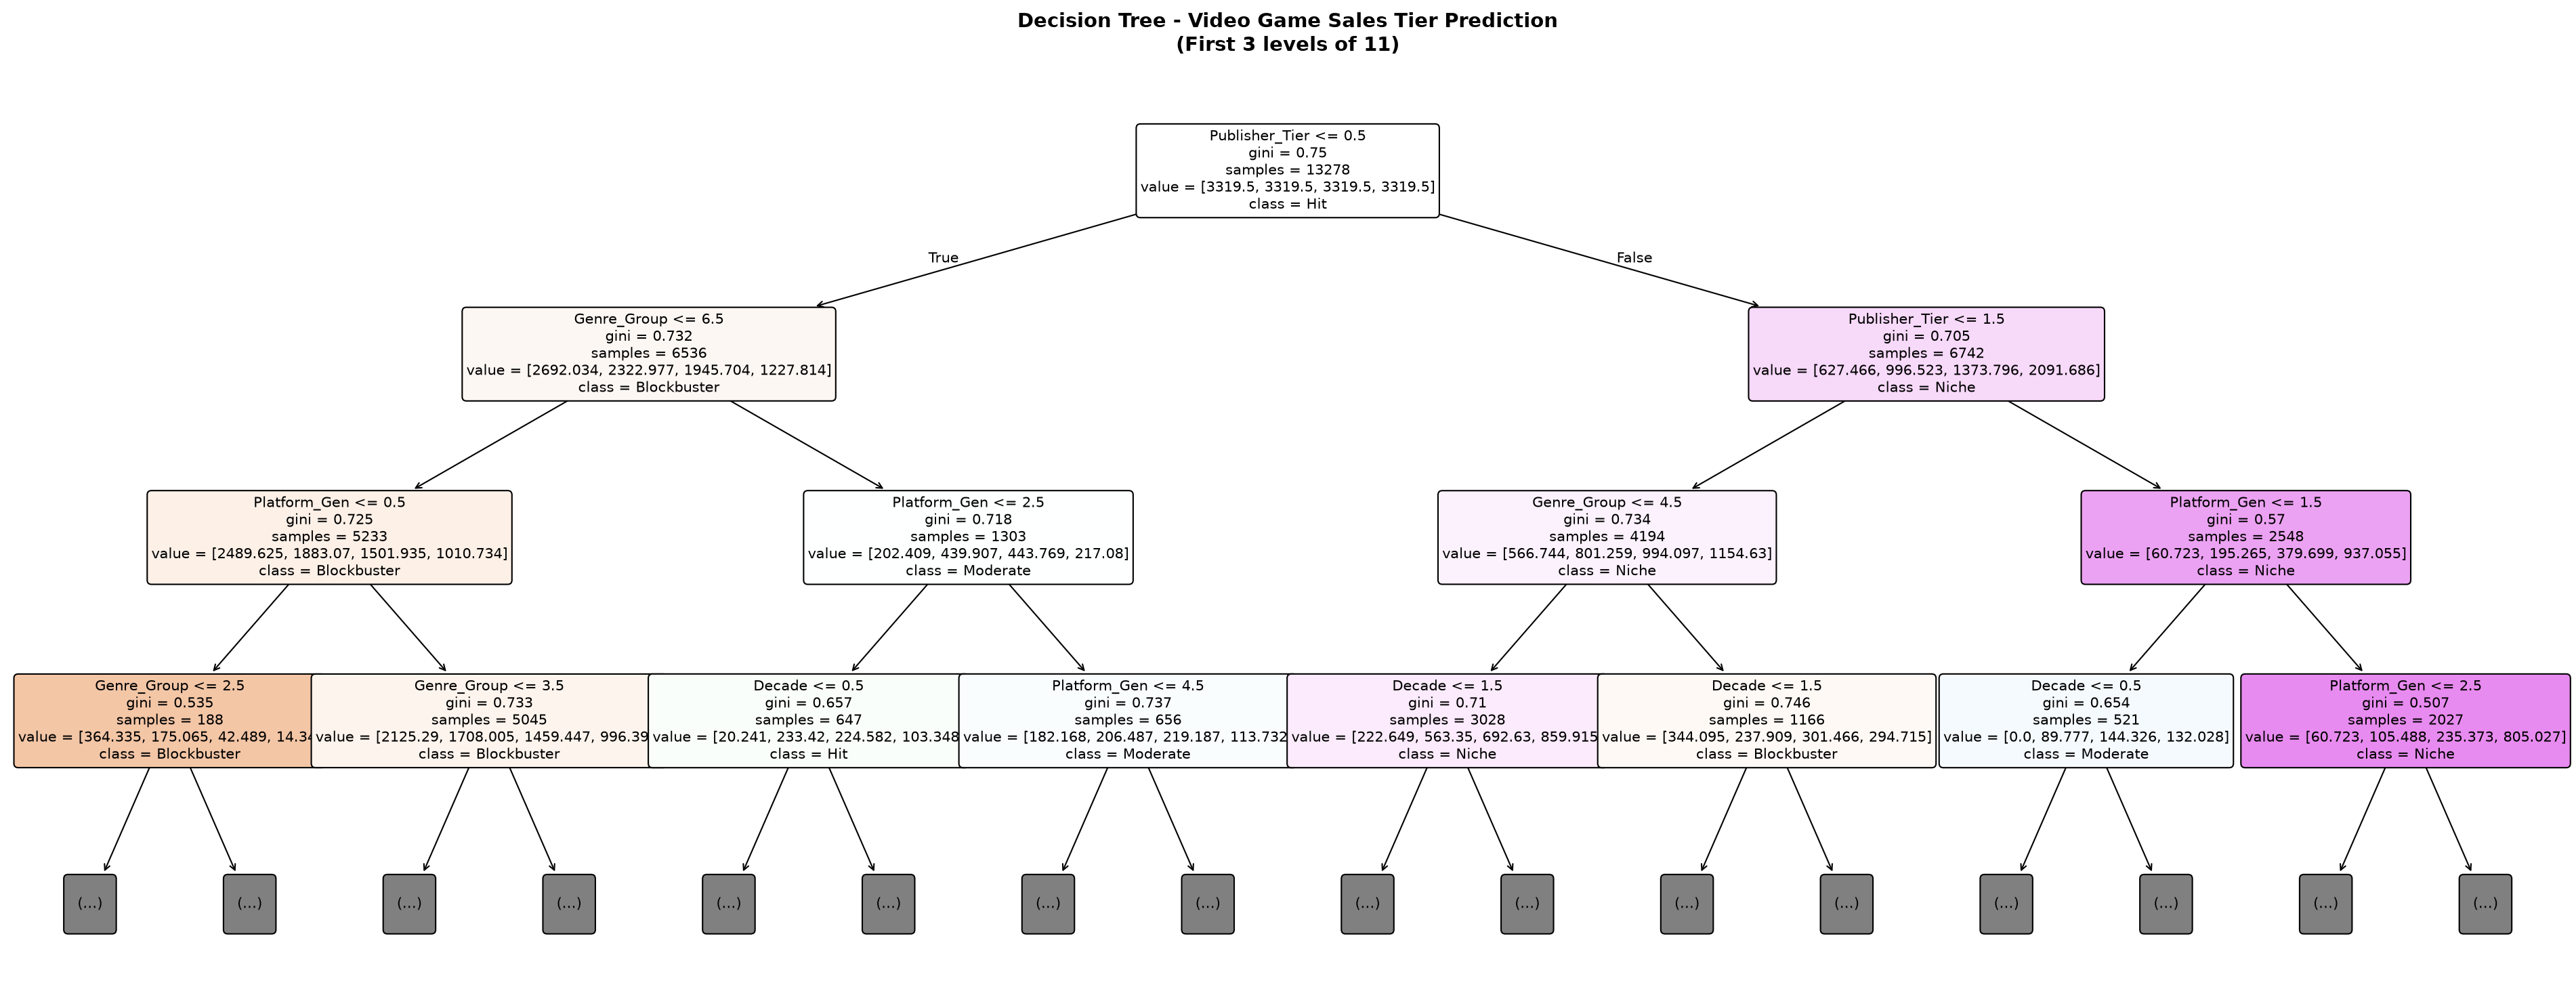
\includegraphics[width=\linewidth]{decision_tree_plot}
  \caption{Decision Tree visualization (first 3 levels).}
\end{figure}

\subsection{Logistic Regression}

Logistic Regression with \texttt{class\_weight="balanced"} and the best \texttt{C} selected by \texttt{GridSearchCV} (\texttt{C}=0.01)
produced results comparable to the balanced Decision Tree: 40\% accuracy and 0.41 balanced accuracy. It recalled 68\% of
\textit{Blockbuster} games but only 16\% of \textit{Hit} games, and it frequently over-predicts \textit{Blockbuster} (low precision).
Table~\ref{tab:results} summarizes the test-set metrics of all models.

\begin{table}[ht]
  \caption{Test-set metrics. Naive Bayes predicts a different target (8 genre groups), so it is not directly comparable.}
  \label{tab:results}
  \begin{tabular}{lccc}
    \toprule
    Model & Accuracy & Bal. acc. & Macro F1 \\
    \midrule
    Decision Tree & 0.565 & 0.331 & 0.325 \\
    Decision Tree (balanced) & 0.396 & 0.406 & 0.300 \\
    Logistic Regression (balanced) & 0.399 & 0.411 & 0.287 \\
    Naive Bayes (genre) & 0.276 & 0.181 & 0.146 \\
    \bottomrule
  \end{tabular}
\end{table}

The confusion matrix in the following figure shows the distribution of correct and incorrect predictions across all four classes.

\begin{figure}[ht]
  \centering
  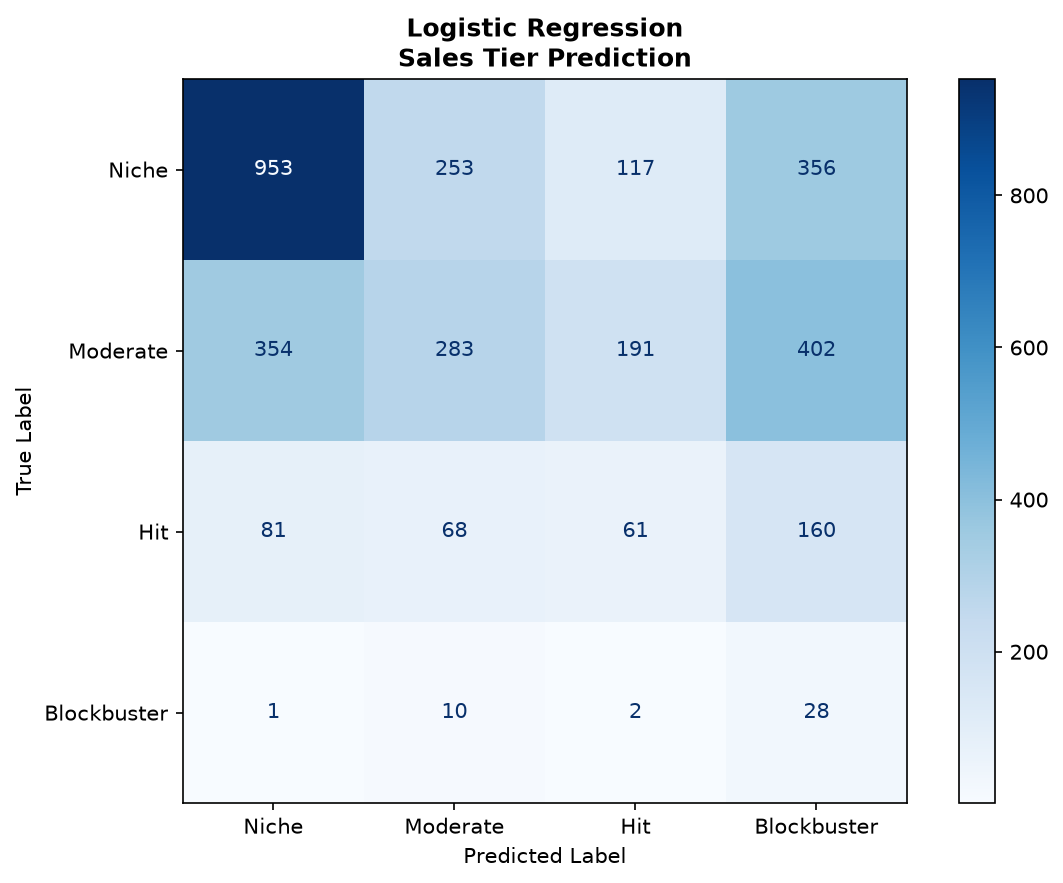
\includegraphics[width=\linewidth]{lr_confusion_matrix}
  \caption{Confusion matrix for Logistic Regression.}
  \label{fig:lr_cm}
\end{figure}

\subsection{Naive Bayes}

The Naive Bayes model (best \texttt{alpha}=5) achieved 28\% accuracy on \texttt{Genre\_Group} prediction, with four of the eight genre classes receiving zero recall
(\textit{Misc}, \textit{Racing}, \textit{Role-Playing}, \textit{Shooter}). The confusion matrix is shown in Figure~\ref{fig:nb_cm}.

\begin{figure}[ht]
  \centering
  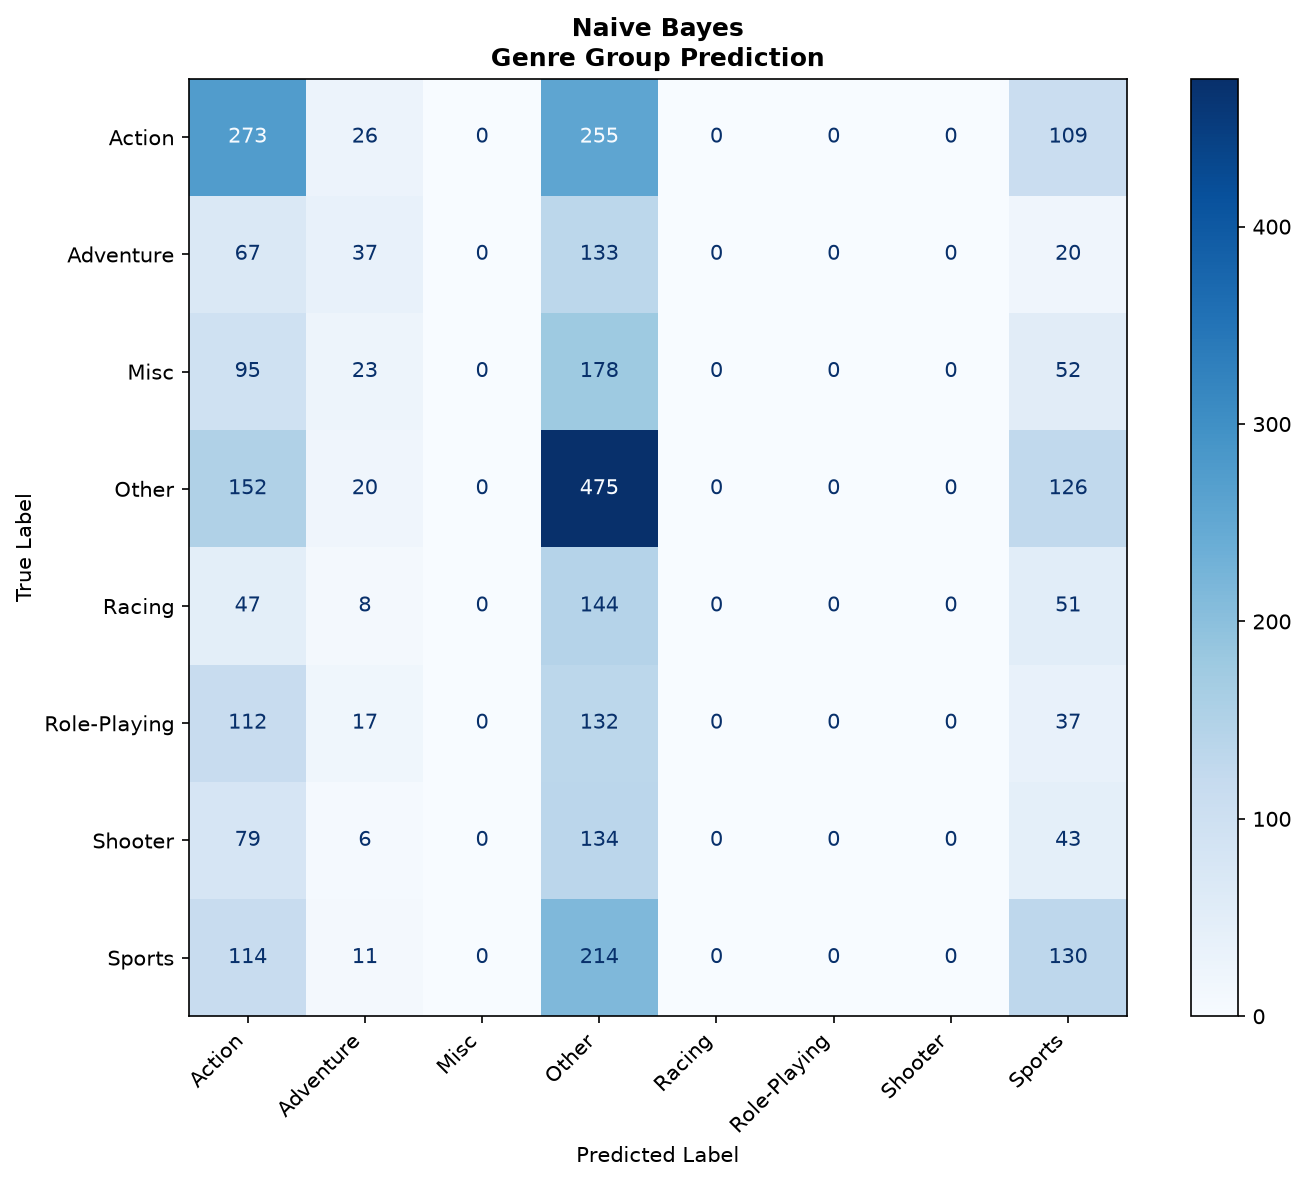
\includegraphics[width=\linewidth]{nb_confusion_matrix}
  \caption{Confusion matrix for Naive Bayes.}
  \label{fig:nb_cm}
\end{figure}

\section{Discussion}

\subsection{Class Imbalance}

Class imbalance was the dominant challenge across all three models. In both the Decision Tree and Logistic Regression, applying
\texttt{class\_weight="balanced"} forced the models to give equal penalty to misclassifying rare classes at the cost of overall accuracy.
Without weighting, a model trained on an imbalanced dataset tends to just learn to predict the majority class.
For the same reason, the weighted models were tuned with balanced accuracy instead of plain accuracy.

\section{Conclusions}

This project trained and evaluated three machine learning classifiers on the vgsales dataset. The Decision Tree and Logistic Regression
demonstrated moderate ability to predict \texttt{Sales\_Tier} from engineered categorical features, with class weighting improving
fairness at the cost of overall accuracy. Naive Bayes achieved low accuracy on genre prediction, primarily due to violated independence assumptions.

The results underscore three broader lessons: (1) feature engineering can sometimes limit a model's performance; (2) accuracy alone
is a misleading metric under class imbalance; and (3) a model that fails informatively is often more valuable for learning than one that
succeeds by chance, as seen in this project. Personally, I found this project to be very interesting and informative.

\begin{thebibliography}{9}
\bibitem{vgsales}
\newblock \texttt{Video Game Sales dataset. Kaggle. } 
\url{https://www.kaggle.com/datasets/gregorut/videogamesales}

\bibitem{sklearn_labelencoder}
scikit-learn developers.
\newblock \texttt{sklearn.preprocessing.LabelEncoder}
\newblock 2025.
\newblock \url{https://scikit-learn.org/stable/modules/generated/sklearn.preprocessing.LabelEncoder.html}

\bibitem{sklearn_onehotencoder}
scikit-learn developers.
\newblock \texttt{sklearn.preprocessing.OneHotEncoder}
\newblock 2025.
\newblock \url{https://scikit-learn.org/stable/modules/generated/sklearn.preprocessing.OneHotEncoder.html}

\bibitem{sklearn_ordinalencoder}
scikit-learn developers.
\newblock \texttt{sklearn.preprocessing.OrdinalEncoder}
\newblock 2025.
\newblock \url{https://scikit-learn.org/stable/modules/generated/sklearn.preprocessing.OrdinalEncoder.html}

\bibitem{gfg_imbalanced_dt}
GeeksforGeeks.
\newblock Training a decision tree against unbalanced data.
\newblock \textit{GeeksforGeeks - Machine Learning}, Nov. 2024.
\newblock \url{https://www.geeksforgeeks.org/machine-learning/training-a-decision-tree-against-unbalanced-data/}

\bibitem{gfg_multiclass_lr}
GeeksforGeeks.
\newblock Multiclass logistic regression.
\newblock \textit{GeeksforGeeks - Artificial Intelligence}, Aug. 2025.
\newblock \url{https://www.geeksforgeeks.org/artificial-intelligence/multiclass-logistic-regression/}

\end{thebibliography}

\end{document}